\documentclass[border=4pt]{standalone}

\usepackage{amsmath}
\usepackage{tikz}
\usepackage{mathdots}
\usepackage{yhmath}
\usepackage{cancel}
\usepackage{color}
\usepackage{siunitx}
\usepackage{array}
\usepackage{multirow}
\usepackage{amssymb}
\usepackage{gensymb}
\usepackage{tabularx}
\usepackage{booktabs}
\usetikzlibrary{fadings}
\usetikzlibrary{patterns}
\usetikzlibrary{shadows.blur}
\usetikzlibrary{shapes}
 

\begin{document}




\tikzset{every picture/.style={line width=0.75pt}} %set default line width to 0.75pt        

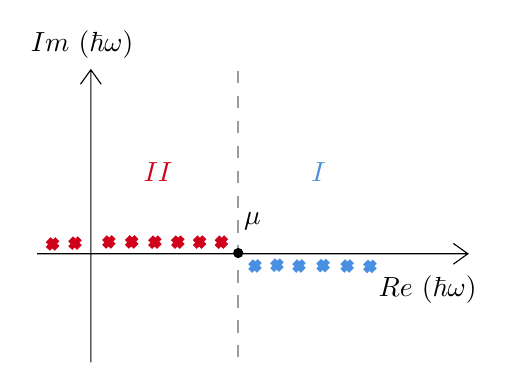
\begin{tikzpicture}[x=0.75pt,y=0.75pt,yscale=-1,xscale=1]
%uncomment if require: \path (0,300); %set diagram left start at 0, and has height of 300

%Shape: Axis 2D [id:dp14009442521926418] 
\draw  (43.6,140.4) -- (251.1,140.4)(69.44,51.73) -- (69.44,192.73) (244.1,135.4) -- (251.1,140.4) -- (244.1,145.4) (64.44,58.73) -- (69.44,51.73) -- (74.44,58.73)  ;
%Straight Lines [id:da3953383606412795] 
\draw [color={rgb, 255:red, 155; green, 155; blue, 155 }  ,draw opacity=1 ] [dash pattern={on 4.5pt off 4.5pt}]  (140.33,52.33) -- (140.33,190.33) ;
%Shape: Circle [id:dp5847082764786693] 
\draw  [color={rgb, 255:red, 0; green, 0; blue, 0 }  ,draw opacity=1 ][fill={rgb, 255:red, 0; green, 0; blue, 0 }  ,fill opacity=1 ] (140.37,137.87) .. controls (141.57,137.83) and (142.56,138.77) .. (142.6,139.97) .. controls (142.63,141.17) and (141.69,142.16) .. (140.5,142.2) .. controls (139.3,142.23) and (138.3,141.29) .. (138.27,140.1) .. controls (138.23,138.9) and (139.17,137.9) .. (140.37,137.87) -- cycle ;
%Shape: Cross [id:dp042349247236526555] 
\draw  [color={rgb, 255:red, 208; green, 2; blue, 27 }  ,draw opacity=1 ][fill={rgb, 255:red, 208; green, 2; blue, 27 }  ,fill opacity=1 ] (75.22,133.77) -- (77.16,131.81) -- (78.32,132.95) -- (79.46,131.79) -- (81,133.31) -- (79.86,134.46) -- (81.01,135.6) -- (79.07,137.57) -- (77.92,136.43) -- (76.78,137.59) -- (75.24,136.07) -- (76.38,134.91) -- cycle ;
%Shape: Cross [id:dp18382615307407568] 
\draw  [color={rgb, 255:red, 208; green, 2; blue, 27 }  ,draw opacity=1 ][fill={rgb, 255:red, 208; green, 2; blue, 27 }  ,fill opacity=1 ] (97.42,133.87) -- (99.36,131.91) -- (100.52,133.05) -- (101.66,131.89) -- (103.2,133.41) -- (102.06,134.56) -- (103.21,135.7) -- (101.27,137.67) -- (100.12,136.53) -- (98.98,137.69) -- (97.44,136.17) -- (98.58,135.01) -- cycle ;
%Shape: Cross [id:dp4933448690304838] 
\draw  [color={rgb, 255:red, 208; green, 2; blue, 27 }  ,draw opacity=1 ][fill={rgb, 255:red, 208; green, 2; blue, 27 }  ,fill opacity=1 ] (86.22,133.77) -- (88.16,131.81) -- (89.32,132.95) -- (90.46,131.79) -- (92,133.31) -- (90.86,134.46) -- (92.01,135.6) -- (90.07,137.57) -- (88.92,136.43) -- (87.78,137.59) -- (86.24,136.07) -- (87.38,134.91) -- cycle ;
%Shape: Cross [id:dp02384410643472612] 
\draw  [color={rgb, 255:red, 208; green, 2; blue, 27 }  ,draw opacity=1 ][fill={rgb, 255:red, 208; green, 2; blue, 27 }  ,fill opacity=1 ] (58.92,134.37) -- (60.86,132.41) -- (62.02,133.55) -- (63.16,132.39) -- (64.7,133.91) -- (63.56,135.06) -- (64.71,136.2) -- (62.77,138.17) -- (61.62,137.03) -- (60.48,138.19) -- (58.94,136.67) -- (60.08,135.51) -- cycle ;
%Shape: Cross [id:dp6586653245420309] 
\draw  [color={rgb, 255:red, 208; green, 2; blue, 27 }  ,draw opacity=1 ][fill={rgb, 255:red, 208; green, 2; blue, 27 }  ,fill opacity=1 ] (129.42,133.87) -- (131.36,131.91) -- (132.52,133.05) -- (133.66,131.89) -- (135.2,133.41) -- (134.06,134.56) -- (135.21,135.7) -- (133.27,137.67) -- (132.12,136.53) -- (130.98,137.69) -- (129.44,136.17) -- (130.58,135.01) -- cycle ;
%Shape: Cross [id:dp9681320516669241] 
\draw  [color={rgb, 255:red, 208; green, 2; blue, 27 }  ,draw opacity=1 ][fill={rgb, 255:red, 208; green, 2; blue, 27 }  ,fill opacity=1 ] (108.42,133.87) -- (110.36,131.91) -- (111.52,133.05) -- (112.66,131.89) -- (114.2,133.41) -- (113.06,134.56) -- (114.21,135.7) -- (112.27,137.67) -- (111.12,136.53) -- (109.98,137.69) -- (108.44,136.17) -- (109.58,135.01) -- cycle ;
%Shape: Cross [id:dp8501906854566981] 
\draw  [color={rgb, 255:red, 208; green, 2; blue, 27 }  ,draw opacity=1 ][fill={rgb, 255:red, 208; green, 2; blue, 27 }  ,fill opacity=1 ] (118.92,133.87) -- (120.86,131.91) -- (122.02,133.05) -- (123.16,131.89) -- (124.7,133.41) -- (123.56,134.56) -- (124.71,135.7) -- (122.77,137.67) -- (121.62,136.53) -- (120.48,137.69) -- (118.94,136.17) -- (120.08,135.01) -- cycle ;
%Shape: Cross [id:dp6035980848041802] 
\draw  [color={rgb, 255:red, 208; green, 2; blue, 27 }  ,draw opacity=1 ][fill={rgb, 255:red, 208; green, 2; blue, 27 }  ,fill opacity=1 ] (48.12,134.77) -- (50.06,132.81) -- (51.22,133.95) -- (52.36,132.79) -- (53.9,134.31) -- (52.76,135.46) -- (53.91,136.6) -- (51.97,138.57) -- (50.82,137.43) -- (49.68,138.59) -- (48.14,137.07) -- (49.28,135.91) -- cycle ;
%Shape: Cross [id:dp3220738635703211] 
\draw  [color={rgb, 255:red, 74; green, 144; blue, 226 }  ,draw opacity=1 ][fill={rgb, 255:red, 74; green, 144; blue, 226 }  ,fill opacity=1 ] (145.62,145.37) -- (147.56,143.41) -- (148.72,144.55) -- (149.86,143.39) -- (151.4,144.91) -- (150.26,146.06) -- (151.41,147.2) -- (149.47,149.17) -- (148.32,148.03) -- (147.18,149.19) -- (145.64,147.67) -- (146.78,146.51) -- cycle ;
%Shape: Cross [id:dp32064688432408217] 
\draw  [color={rgb, 255:red, 74; green, 144; blue, 226 }  ,draw opacity=1 ][fill={rgb, 255:red, 74; green, 144; blue, 226 }  ,fill opacity=1 ] (201.02,145.57) -- (202.96,143.61) -- (204.12,144.75) -- (205.26,143.59) -- (206.8,145.11) -- (205.66,146.26) -- (206.81,147.4) -- (204.87,149.37) -- (203.72,148.23) -- (202.58,149.39) -- (201.04,147.87) -- (202.18,146.71) -- cycle ;
%Shape: Cross [id:dp23136544150496174] 
\draw  [color={rgb, 255:red, 74; green, 144; blue, 226 }  ,draw opacity=1 ][fill={rgb, 255:red, 74; green, 144; blue, 226 }  ,fill opacity=1 ] (190.02,145.37) -- (191.96,143.41) -- (193.12,144.55) -- (194.26,143.39) -- (195.8,144.91) -- (194.66,146.06) -- (195.81,147.2) -- (193.87,149.17) -- (192.72,148.03) -- (191.58,149.19) -- (190.04,147.67) -- (191.18,146.51) -- cycle ;
%Shape: Cross [id:dp9310933854126184] 
\draw  [color={rgb, 255:red, 74; green, 144; blue, 226 }  ,draw opacity=1 ][fill={rgb, 255:red, 74; green, 144; blue, 226 }  ,fill opacity=1 ] (178.42,145.17) -- (180.36,143.21) -- (181.52,144.35) -- (182.66,143.19) -- (184.2,144.71) -- (183.06,145.86) -- (184.21,147) -- (182.27,148.97) -- (181.12,147.83) -- (179.98,148.99) -- (178.44,147.47) -- (179.58,146.31) -- cycle ;
%Shape: Cross [id:dp6080069791905443] 
\draw  [color={rgb, 255:red, 74; green, 144; blue, 226 }  ,draw opacity=1 ][fill={rgb, 255:red, 74; green, 144; blue, 226 }  ,fill opacity=1 ] (166.82,145.37) -- (168.76,143.41) -- (169.92,144.55) -- (171.06,143.39) -- (172.6,144.91) -- (171.46,146.06) -- (172.61,147.2) -- (170.67,149.17) -- (169.52,148.03) -- (168.38,149.19) -- (166.84,147.67) -- (167.98,146.51) -- cycle ;
%Shape: Cross [id:dp3666698417869789] 
\draw  [color={rgb, 255:red, 74; green, 144; blue, 226 }  ,draw opacity=1 ][fill={rgb, 255:red, 74; green, 144; blue, 226 }  ,fill opacity=1 ] (156.22,144.97) -- (158.16,143.01) -- (159.32,144.15) -- (160.46,142.99) -- (162,144.51) -- (160.86,145.66) -- (162.01,146.8) -- (160.07,148.77) -- (158.92,147.63) -- (157.78,148.79) -- (156.24,147.27) -- (157.38,146.11) -- cycle ;

% Text Node
\draw (39.27,31.73) node [anchor=north west][inner sep=0.75pt]    {$Im\ ( \hbar \omega )$};
% Text Node
\draw (206.8,149.51) node [anchor=north west][inner sep=0.75pt]    {$Re\ ( \hbar \omega )$};
% Text Node
\draw (93.6,95.2) node [anchor=north west][inner sep=0.75pt]  [color={rgb, 255:red, 208; green, 2; blue, 27 }  ,opacity=1 ]  {$II$};
% Text Node
\draw (174.4,95.4) node [anchor=north west][inner sep=0.75pt]  [color={rgb, 255:red, 74; green, 144; blue, 226 }  ,opacity=1 ]  {$I$};
% Text Node
\draw (142,119.2) node [anchor=north west][inner sep=0.75pt]    {$\mu $};


\end{tikzpicture}

\end{document}
